\documentclass[a4paper,11pt]{article}
\usepackage{Sweave}
\title{Project Parallel Programming \\ IPL Rubik's Cube Solver}
\author{ Linus Schoemaker (lsr450/1961667)}
\begin{document}

\maketitle

\section{Introduction}

This report describes the implementation of a parallel Rubik's cube solver using the Ibis Portability layer. We will start by outlining the approach used, and why this implementation was chosen. We will then demonstrate the speedups achieved by using this parallel algorithm as compared to the sequential version. Finally we will describe some other approaches tried, and why we believe our version is better.

\section{Parallel Algorithm}

To understand the parallel version of the algorithm used here we must first understand the sequential version.
In the sequential algorithm provided, a Rubik's cube was either randomly generated or read from file. The generated cube could be specified by setting the number of sides of the cube and number of random twists to perform on the starting solved cube. 

Once the algorithm received a cube as input, it would generate all possible new cubes from the starting cube. It would then check if any of these children was a solved cube. If not, it would start over, searching one level deeper. This would mean generating all children of the original cube, and then all possible children of the newly generated cubes. The algorithm would continue increasing the depth of search until a solution was found.

This algorithm is an iterative deepening depth-first search algorithm. This is an important observation when it comes to implementing the parallel version. 


The parallel implementation of the algorithm is fairly straightforward. Out of the available nodes we elect one server, turning the rest of the nodes into clients. The server then creates all possible children of the original input cube. It evenly divides the amount of cubes over the amount of nodes, and sends each nodes its share of cubes. This means each node has one or more subtrees to search through. 

The nodes then search through their subtree(s) in the same way the original algorithm did. When a node finds a solution, it sends it back to the server. Once the server receives this answer, it broadcasts the level on which the solution was found to all nodes. This stops nodes from searching past a level at which a solution was found by another node. After all, we are only looking for the smallest solution. 

The nodes continuously poll the server whether a new lowest level has been found. If it has, a node will only search up to and including this level, as its subtree might also contain a solution at this level. This is because we also need to know \emph{how many} solutions there are at the lowest possible level. 

Nodes finish either once they have found a solution, or they have not but would need to look past a level at which a solution has been found by another node. Once finished nodes send back their answer (x solutions at level y, or 0 solutions) to the server.

The server then adds up all solutions of the lowest level, and prints them for the user. 

\section{Speedup}

\noindent

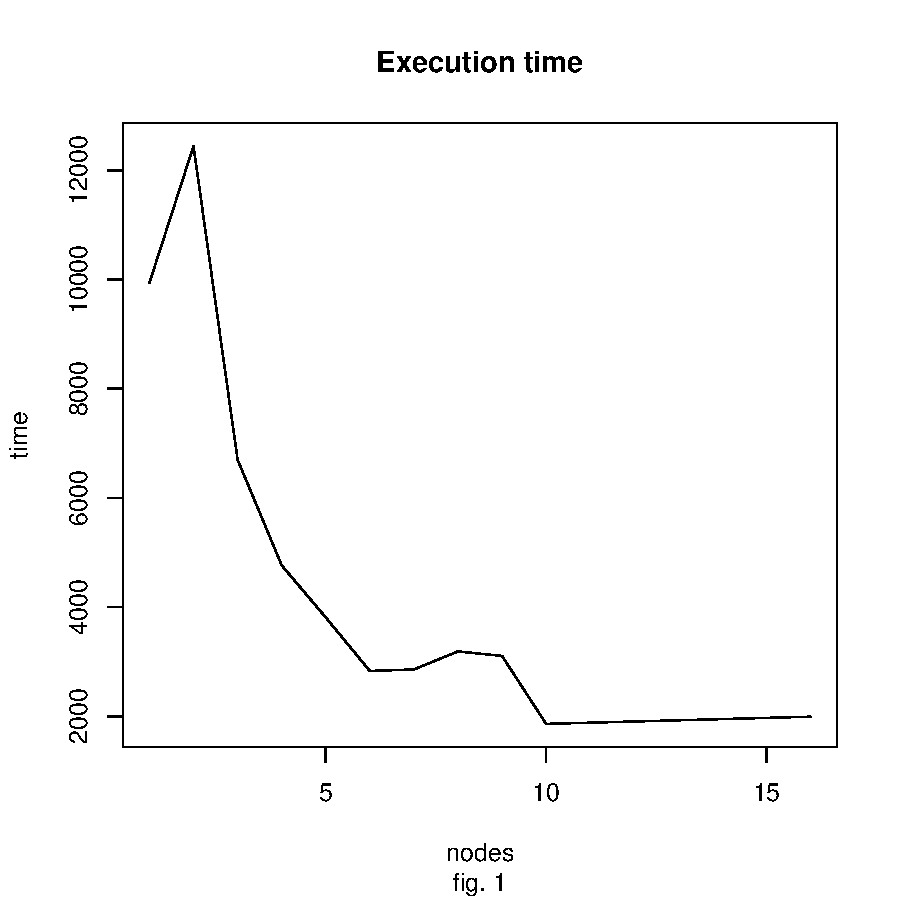
\includegraphics{report-001}

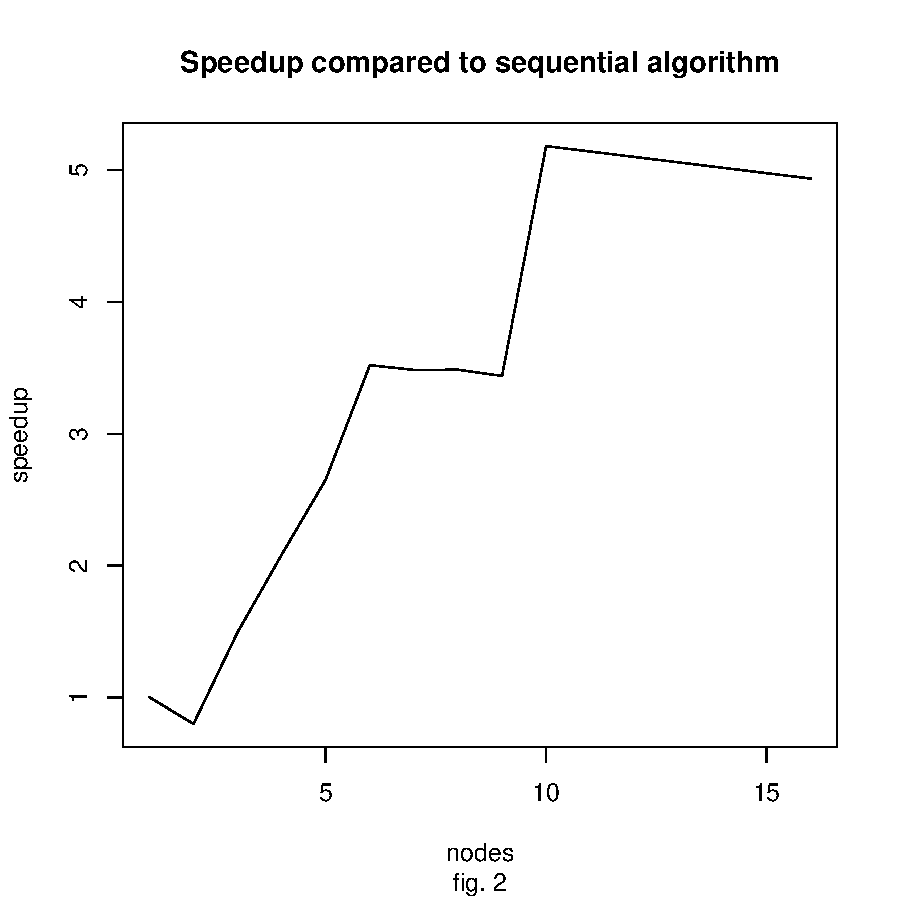
\includegraphics{report-002}

These figures illustrate the speedup achieved by parallelizing the algorithm. All measurements were done by randomly generating a cube twisted 11 times, using a random seed of 5. Two possible solutions were found after 7 twists. All values are the mean of three measurements, to account for small differences caused by system load etcetera.

Although the speedup is not even remotely linear, there is a clear improvement when using more nodes. When disregarding the performance of the sequential algorithm, doubling the nodes roughly halves the time needed for execution. The difference with the sequential algorithm can mainly be attributed to communication overhead and initialization of the Ibis system. 

The graph contains some irregularities that need an explanation. 

The first is the sharp increase when going from one to two nodes. This can be explained by the fact that when the system uses only one node, the server performs the sequential algorithm, i.e. no communication. When there are two nodes however, one becomes server and one becomes client. The client will then perform almost the same operations as the entire sequential algorithm, but with communication and initialization time added. 

The second is the bump around 8 and 9 nodes. This can be explained by the fact that the server generates 12 child cubes, which is tough to divide over 9 nodes. This means some nodes will receive only one cube, while some get two. Because nodes must search their entire tree up to a certain level, this means performance doesn't really increase. 

The last is the fact that after 10 nodes there is little to no improvement. This can also be explained by the fact that the server only generates 12 cubes: after 13 nodes, all extra nodes do nothing!


\section{Difficulties}

The largest problem with finding a solution in this situation was search overhead. In the first version of the algorithm it generated the children of the input cube, put them in a queue and distributed them among the workers cube by cube. Workers would explore the tree generated by their cube until they found a solution. 

This caused a tremendous amount of search overhead: if none of the first nodes could find an optimal solution in their first cube they might search several levels deeper than necessary. Each level increases the input size by a factor of 12 when using a three-sided cube, causing the data, and processing time, to grow exponentially. 

To mitigate this problem, there are two solutions: either all nodes report their findings back to the server after searching one level, after which the server sends them a new cube. This would imply a massive communication overhead. The other solution, which was chosen here, was to immediately distribute all the data among the nodes, meaning one node could receive multiple cubes. The node would then search the tree of a cube to a certain level, and then move on to the next. If no answer was found in any of the trees, it would increase the search level and start over. This seemed like the most efficient solution. A drawback is that when there are more nodes than cubes generated by the server, some nodes are not used. A solution here would be to have the server generate more cubes by going one level deeper in the tree. 


\end{document}

